\chapter{ארכיטקטורת השנאי}

\section{יסודות המנגנון-קשב}

מנגנון הקשב (\textenglish{Attention Mechanism}) מהווה את הלב הפועם של ארכיטקטורת השנאי (\textenglish{Transformer}). בניגוד לרשתות נוירונים רקורנטיות המעבדות נתונים ברצף ודורשות זמן חישוב ריבועי בקנה מידה של אורך הרצף, השנאי מאפשר עיבוד מקביל של כל התאימים בו-זמנית. כפי שתואר ב-\cite{vaswani2017attention}, מנגנון הקשב מחשב מטריצת משקלים המשדכת כל אלמנט בקלט עם כל אלמנט אחר בו בשלב יחיד.

הנוסחה החישובית למנגנון הקשב היא:

\begin{equation}
\text{Attention}(Q, K, V) = \text{softmax}\left(\frac{QK^T}{\sqrt{d_k}}\right)V
\end{equation}

כאשר \(Q\) (\textenglish{Query}), \(K\) (\textenglish{Key}), ו-\(V\) (\textenglish{Value}) הן מטריצות המתקבלות מהשכבות הקודמות. הגורם \(\sqrt{d_k}\) משמש לנרמול כדי לשמור על יציבות מספרית וקצב ההתכנסות בהדרכה. לאחר חישוב פונקציית ה-\textenglish{softmax}, המשקלים מוחלים על מטריצת הערכים כדי לייצר פלט קשוב. מורכבות הזמן של פעולת ה-\textenglish{self-attention} היא \textenglish{O(n\textsuperscript{2}·d)} כאשר \textenglish{n} הוא אורך הרצף ו-\textenglish{d} הוא ממד ההטמעה --- יתרון ברור על פני ה-\textenglish{RNN} בו הזמן הסדרתי גדל לינארית אך ללא מקביליות.

\begin{figure}[H]
\centering
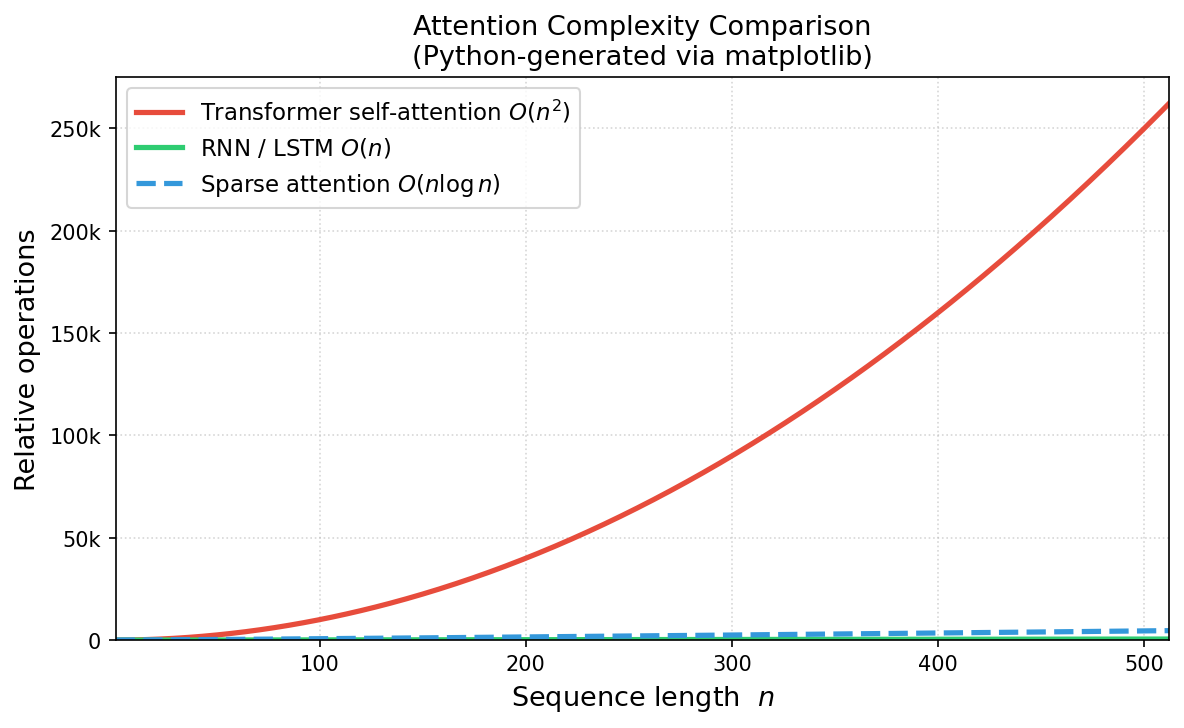
\includegraphics[width=0.8\textwidth]{assets/attention_complexity.png}
\caption{\textenglish{Attention Complexity}}
\label{fig:attention_complexity}
\end{figure}

\section{ארכיטקטורת \textenglish{Multi-Head Attention}}

בעוד שמנגנון קשב יחיד יכול לתפוס קשרים מסוימים בין נתונים, השנאי משתמש בעשרות ראשי קשב (\textenglish{Attention Heads}) במקביל. כל ראש מאומן באופן עצמאי וחוקר היבטים שונים של הנתונים. השימוש בראשים מרובים מגביר את יכולת המודל ללמוד תבניות מורכבות וליצור ייצוג עשיר של הקלט.

כמתואר ב-\cite{devlin2019bert}, ארכיטקטורת \textenglish{Multi-Head Attention} מאפשרת למודל להתמקד בחלקים שונים של הרצף בו-זמנית. לדוגמה, חלק מהראשים עשויים ללמוד קשרים תחביריים (\textenglish{Syntactic Relations}) בעוד שאחרים לומדים קשרים סמנטיים (\textenglish{Semantic Relations}). המשוואה המתארת \textenglish{Multi-Head Attention} היא:

\begin{equation}
\text{MultiHead}(Q, K, V) = \text{Concat}(\text{head}_1, \ldots, \text{head}_h)W^O
\end{equation}

כאשר כל \textenglish{head} מחושב לפי:
\begin{equation}
\text{head}_i = \text{Attention}(QW_i^Q,\; KW_i^K,\; VW_i^V)
\end{equation}

\section{השכבות הלינאריות וההנדסה הפנימית}

לאחר שכבת \textenglish{Multi-Head Attention}, הנתונים עוברים דרך רשת נוירונים עמוקה בעלת שכבות לינאריות עם פונקציית הפעלה לא-לינאית (בדרך כלל \textenglish{ReLU} או \textenglish{GELU}). שכבה זו, המכונה \textenglish{Feed-Forward Network} (\textenglish{FFN}), מייצגת הנדסה פנימית משמעותית. כל יחידה בשכבה הלינאארית הראשונה לומדת שילובים של תכונות הקלט, מה שמאפשר למודל לתפוס קשרים לא-לינאריים מורכבים.

הנוסחה של \textenglish{FFN} היא:

\begin{equation}
\text{FFN}(x) = \max(0, xW_1 + b_1)W_2 + b_2
\end{equation}

מימד הביניים (\textenglish{Hidden Dimension}) של שכבה זו בדרך כלל גדול פי 4 מממד הפלט, כפי שנחקר ב-\cite{brown2020language}. בחקר יסודי זה, הוכח כי הגדלת מימד הביניים משפרת את ביצועי המודל, אם כי בעלות חישובית מוגברת.

\section{נורמליזציה וחיבורים שיוריים}

חיבורים שיוריים (\textenglish{Residual Connections}) ונרמליזציה בשכבה (\textenglish{Layer Normalization}) משמשים מטבעות חיוני בארכיטקטורת השנאי. כל תת-שכבה (\textenglish{sub-layer}) מכילה חיבור שיורי המוסיף את הקלט המקורי לפלט המעובד:

\begin{equation}
\text{LayerNorm}(x + \text{SubLayer}(x))
\end{equation}

חיבורים אלה מקלים על ההדרכה של מודלים עמוקים מאוד על ידי הבטחת שדרגות גדול גם בשכבות העמוקות. נרמליזציה בשכבה משמשת לשיפור יציבות האימון וצמצום התלות בקצב הלמידה, כפי שהוכח ב-\cite{radford2019language}.

\section{קידוד מיקום וטבלאות הטמעה}

בניגוד לרשתות נוירונים רקורנטיות המעבדות רצף אחרי רצף, השנאי מעבד את כל הרצף בו-זמנית. לכן, המודל דורש אמצעי לקידוד המידע החיובי של כל אלמנט בתוך הרצף. זה מושג באמצעות \textenglish{Positional Encoding}, המוסיף וקטור תלוי-מיקום לכל הטמעה של אלמנט.

הנוסחה של קידוד המיקום היא:

\begin{equation}
\text{PE}(pos, 2i) = \sin(pos / 10000^{2i/d_{model}})
\end{equation}

\begin{equation}
\text{PE}(pos, 2i+1) = \cos(pos / 10000^{2i/d_{model}})
\end{equation}

כאשר \(pos\) הוא המיקום בתוך הרצף ו-\(i\) הוא האינדקס של הממד בווקטור ההטמעה. בגרסאות מודרניות של שנאים, כמו \textenglish{LLaMA} (\cite{touvron2023llama}), השימוש בקידוד מיקום רוטציוני (\textenglish{Rotary Position Embeddings}) משפר את הטוענות של המודל לרצפים ארוכים.

\section{סיכום ושימוש ב-\textenglish{ELECTRA}}

ארכיטקטורת השנאי הפכה לתשתית למודלים עדכניים של טיפול בשפה טבעית. כמודל ה-\textenglish{ELECTRA} שמתואר ב-\cite{clark2020electra}, הם מצטיינים בימים המשימות של סיווג טקסט וחילוץ מידע. השילוב של מנגנון-קשב, פיד-פורוורד רשתות, קידוד מיקום, ונרמליזציה בשכבה יוצר מודל חזק וניתן להרחבה הגם לבעיות מעבדה קשות ומורכבות.

עם זאת, ארכיטקטורת השנאי אינה הפתרון היחיד לעיבוד רצפים. בפרק הבא נסקור את רשתות \textenglish{LSTM} הרקורנטיות --- הקדמה ההיסטורית לשנאי --- ואת השימוש בהן לחילוץ פרמטרים מאותות סינוסואידליים. ב\-\textenglish{domain} של עיבוד אותות (כגון הפרדת קול ממיזוג), היתרון המיוחד של \textenglish{RNN} הוא עיבוד \emph{מקוון} בו כל דגימה מוזנת ברצף --- גישה המאפשרת עיבוד בזמן-אמת בזיכרון מוגבל, שבו מורכבות \textenglish{O(n\textsuperscript{2})} של השנאי הופכת לגורם מגביל.
